\documentclass[11pt,a4paper]{article}
\usepackage[margin=2.5cm]{geometry}
\usepackage[utf8]{inputenc}
\usepackage[T1]{fontenc}
\usepackage{hyperref}
\renewcommand{\familydefault}{\sfdefault}
\usepackage{helvet}
\pagestyle{empty}
\usepackage[kerning=true]{microtype}
\usepackage{parskip}
\usepackage{sansmath}
\usepackage[font={small, bf}]{caption}
\usepackage[font={small}]{subcaption}
\usepackage{graphicx}
\usepackage{multicol}
\setlength{\abovecaptionskip}{0pt}
\setlength{\floatsep}{10pt}
\setlength{\textfloatsep}{0pt}
\setlength{\intextsep}{0pt}
\setlength{\belowcaptionskip}{0pt}
\setlength{\parindent}{5ex}
\setlength{\parskip}{0pt}
% Feel free to use additional packages for glosses, figures, whatnot.

% The next bit is for reserving sufficient space for authors,
% affiliations, and e-mail address.  No need to change for initial
% anonymous version.  For the final version, replace the
% \toggletrue{anonymous} with \togglefalse{anonymous} to de-anonymize.
\usepackage{etoolbox}
\newtoggle{anonymous}
\togglefalse{anonymous}

\renewcommand{\title}[1]{\textbf{#1}\\}
\newcommand{\authors}[1]{\iftoggle{anonymous}{\phantom{#1}}{#1}\\}
\newcommand{\email}[1]{\iftoggle{anonymous}{\phantom{#1}}{#1}}

\begin{document}

% First page:

% Insert title, authors, affiliations, and e-mail address in the next three lines:

\title{Thick feedback facilitates referential coordination in larger groups}
\authors{Veronica Boyce\textsuperscript{1}, Robert D.  Hawkins\textsuperscript{2}, Noah D. Goodman\textsuperscript{1}, Michael C. Frank\textsuperscript{1}} 
\email{vboyce@stanford.edu;  \textsuperscript{1}Stanford, \textsuperscript{2}Princeton}
\newline
%

% Intro
%TODO citations
Shared referring expressions are necessary for efficient communication; when there are not conventional names for objects, interlocutors create spontaneous ad-hoc expressions. The formation and adoption of these new reference expressions is well-studied in dyadic iterated reference games. Over repetition, a few key phenomena emerge: listeners have high and increasing selection accuracy while speaker's referring expressions shorten as shared conceptualizations result in partner-specific nicknames. These patterns are also found in small groups where a speaker addresses up to 5 listeners at once (Yoon \& Brown Schmidt 2019, Boyce et al. 2022). Here we begin to address what properties of the communication channel support this phenomena and whether they differ by group size.

\textbf{Methods:} We conducted a 2x2 experiment crossing group size (2 or 6 players) with communication channel width. In \textbf{thick} games (maximizing communication and shared knowledge), the same player was the speaker the entire time, the speaker and listeners could send chat messages to the whole group, and all players saw who selected what image and whether it was right. In contrast, in the \textbf{thin} condition, the speaker role rotated each block, only the speaker could send chat messages while listeners were limited to sending 4 emojis to indicate their level of understanding, and each listener only saw feedback on their own selection.
% should we try to justify this

We recruited participants from Prolific to play a real-time communication game implemented in Empirica (Almaatouq et al. 2021). Participants saw 12 tangram figures, with the target highlighted for the speaker The speaker described the target to the listeners using the chat box, and listeners clicked on their selection (Fig 1). Speakers and listeners received feedback at the end of each trial. After all 12 tangrams were described, the process repeated, for a total of 6 blocks (72 referential trials). We ran roughly 40 games in each of the 4 conditions, for a total of 623 participants (160K words). 

% Results

\textbf{Results:} In line with prior work, we found increasing listener accuracy and decreasing utterance lengths over the course of the game (Figs 2A and B). Speakers used fewer words in 2 player games compared to 6 player games independent of block. Both group size and channel width affected listener accuracy: 2 person groups and thick channels had higher accuracies. 

We embedded the speaker's utterances using S-BERT (Reimers \& Gurevych 2020) which mapped the speaker's language on each trial to a vector in a high-dimensional semantic space. We then used cosine similarity between pairs of vectors as a proxy for similarity between pairs of utterances. To look for the emergence of group-specific descriptions, we took cosine similarities between descriptions of the same tangram in the same block in different games. If groups developed partner-specific nicknames, similarity would decrease over time. We found decreasing similarity in 2 player games and 6 player thick games (Fig 2C). The 6 player thin condition showed a much flatter pattern, suggesting less differentiation between games. 

To measure within-group convergence to a shared convention, we treated final block utterances as the ``convention'' and measured the cosine similarity between earlier utterances in the same game for the same tangram to this final convention. Convergence to a convention would mean increasing cosine similarity across blocks. Similarity increased across all conditions; however, thick games increased faster and more strongly, indicating faster convergence to nicknames, while 6-player thin games increased only a little (Fig 2D). 

\textbf{Conclusion:} We examined how group size and communiciation channel width jointly influenced participants performance in an interated reference game. Participants in all conditions improved at the task. However, the 6-player, thin channel games did not show convergence to shared, partner-specific conventions, seen in other conditions. This suggests that some aspects of a thick channel are needed to rescue communication and hold larger groups together, while dyads can make due and form conventions even with constrained communication. 

\newpage

\begin{figure}
	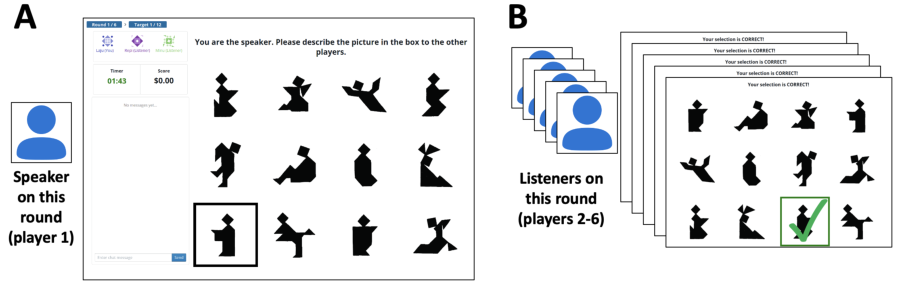
\includegraphics[width=\textwidth]{../images/interface-1.pdf}
	\caption{Schematic of player interface}
\end{figure}

\begin{figure}
	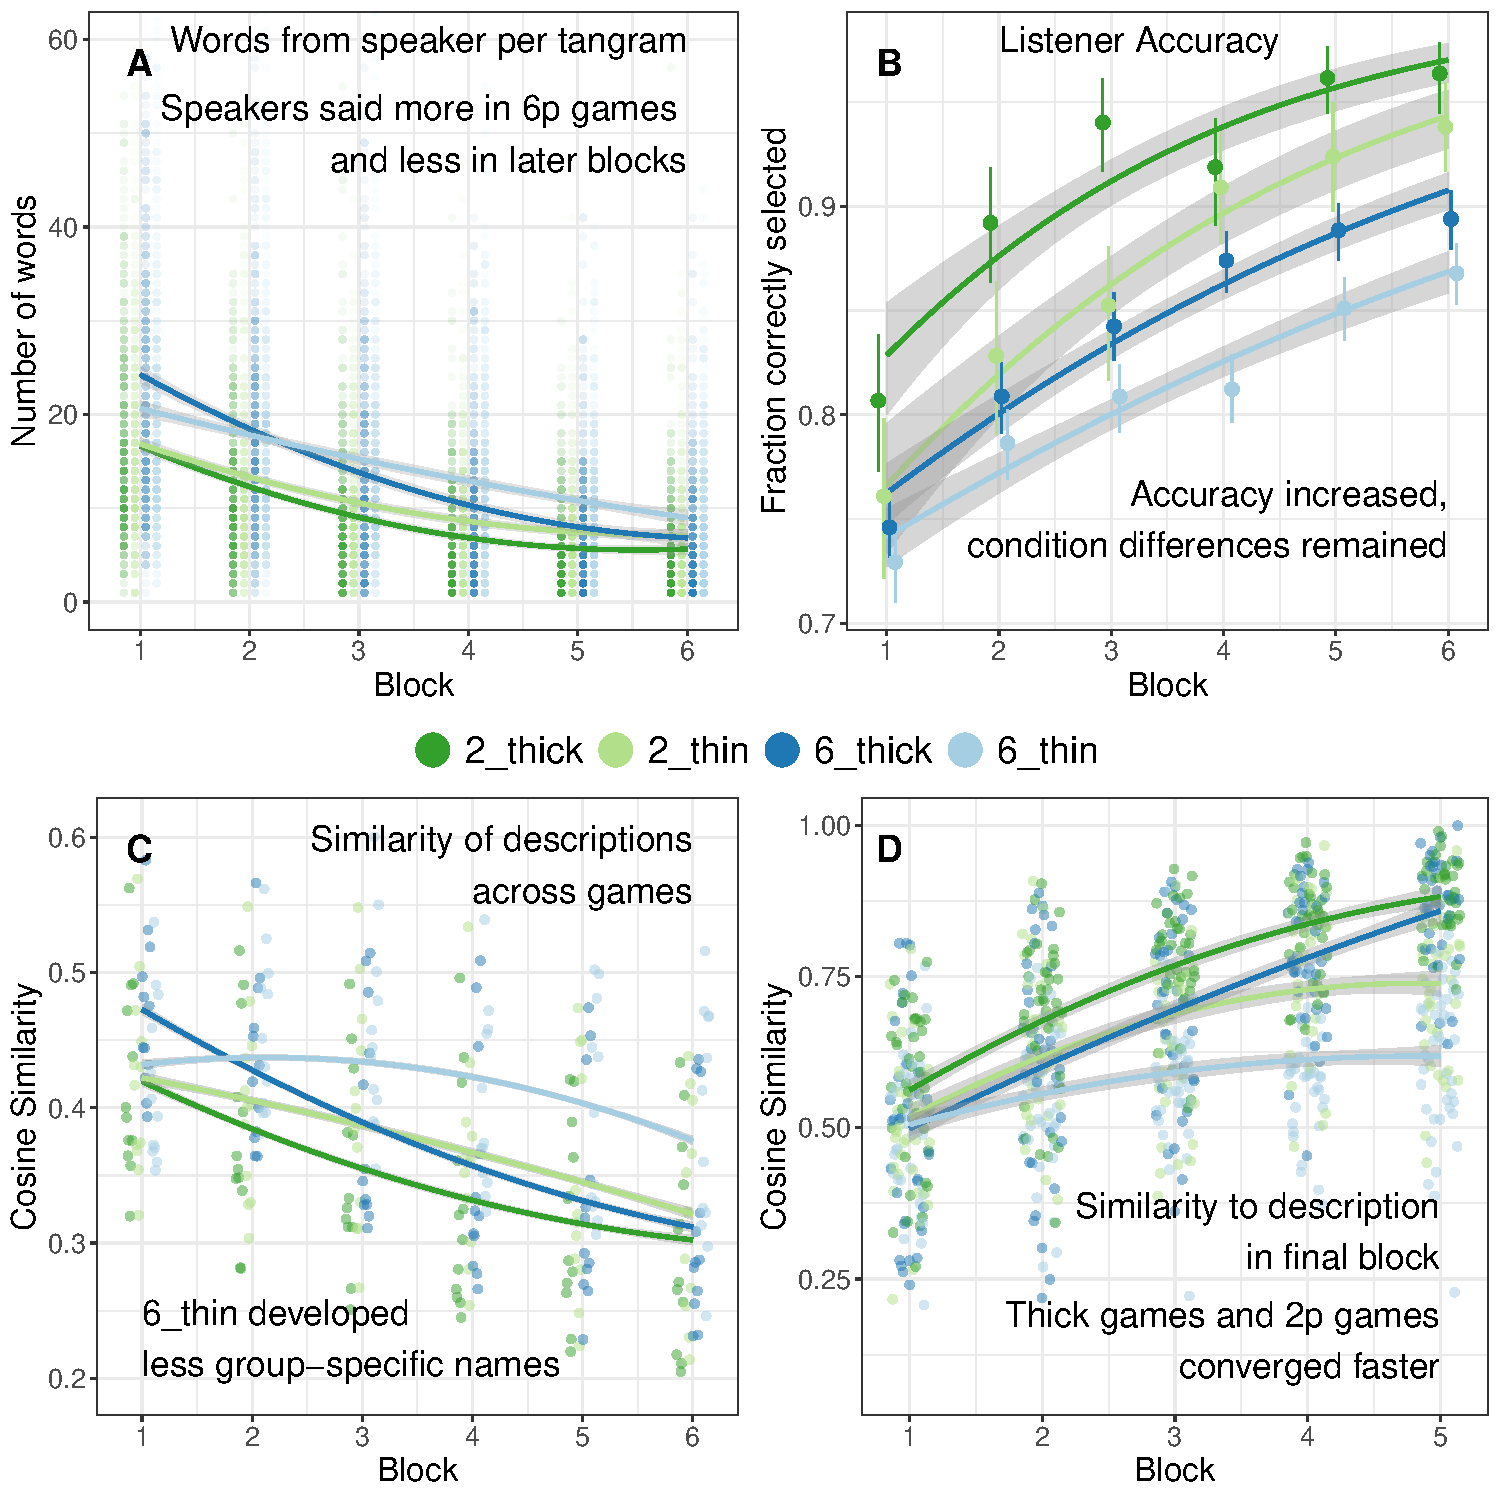
\includegraphics[width=\textwidth]{../images/CAMP1.pdf}
	\caption{Results by condition}
\end{figure}

\begin{figure}\textbf{References:}  Almaatouq, Becker, Houghton, Paton, Watts \& Whiting. Behavioral Research Methods 2021. 
$\bullet$ Boyce, Hawkins, Goodman \& Frank. 44th CogSci 2022. $\bullet$ Reimers \& Gurevych. EMNLP 2020. 
$\bullet$ Yoon \& Brown-Schmidt. Cognitive Science 2019.
  \end{figure}

\end{document}